% Options for packages loaded elsewhere
\PassOptionsToPackage{unicode}{hyperref}
\PassOptionsToPackage{hyphens}{url}
%
\documentclass[
  12pt,
  letterpaper,
  DIV=11,
  numbers=noendperiod]{scrartcl}

\usepackage{amsmath,amssymb}
\usepackage{setspace}
\usepackage{iftex}
\ifPDFTeX
  \usepackage[T1]{fontenc}
  \usepackage[utf8]{inputenc}
  \usepackage{textcomp} % provide euro and other symbols
\else % if luatex or xetex
  \usepackage{unicode-math}
  \defaultfontfeatures{Scale=MatchLowercase}
  \defaultfontfeatures[\rmfamily]{Ligatures=TeX,Scale=1}
\fi
\usepackage{lmodern}
\ifPDFTeX\else  
    % xetex/luatex font selection
    \setmainfont[ItalicFont=EB Garamond Italic,BoldFont=EB Garamond
SemiBold]{EB Garamond Math}
    \setsansfont[]{EB Garamond SemiBold}
  \setmathfont[]{EB Garamond Math}
\fi
% Use upquote if available, for straight quotes in verbatim environments
\IfFileExists{upquote.sty}{\usepackage{upquote}}{}
\IfFileExists{microtype.sty}{% use microtype if available
  \usepackage[]{microtype}
  \UseMicrotypeSet[protrusion]{basicmath} % disable protrusion for tt fonts
}{}
\makeatletter
\@ifundefined{KOMAClassName}{% if non-KOMA class
  \IfFileExists{parskip.sty}{%
    \usepackage{parskip}
  }{% else
    \setlength{\parindent}{0pt}
    \setlength{\parskip}{6pt plus 2pt minus 1pt}}
}{% if KOMA class
  \KOMAoptions{parskip=half}}
\makeatother
\usepackage{xcolor}
\usepackage[left=1in,right=1in,top=1in,bottom=1in]{geometry}
\setlength{\emergencystretch}{3em} % prevent overfull lines
\setcounter{secnumdepth}{5}
% Make \paragraph and \subparagraph free-standing
\makeatletter
\ifx\paragraph\undefined\else
  \let\oldparagraph\paragraph
  \renewcommand{\paragraph}{
    \@ifstar
      \xxxParagraphStar
      \xxxParagraphNoStar
  }
  \newcommand{\xxxParagraphStar}[1]{\oldparagraph*{#1}\mbox{}}
  \newcommand{\xxxParagraphNoStar}[1]{\oldparagraph{#1}\mbox{}}
\fi
\ifx\subparagraph\undefined\else
  \let\oldsubparagraph\subparagraph
  \renewcommand{\subparagraph}{
    \@ifstar
      \xxxSubParagraphStar
      \xxxSubParagraphNoStar
  }
  \newcommand{\xxxSubParagraphStar}[1]{\oldsubparagraph*{#1}\mbox{}}
  \newcommand{\xxxSubParagraphNoStar}[1]{\oldsubparagraph{#1}\mbox{}}
\fi
\makeatother


\providecommand{\tightlist}{%
  \setlength{\itemsep}{0pt}\setlength{\parskip}{0pt}}\usepackage{longtable,booktabs,array}
\usepackage{calc} % for calculating minipage widths
% Correct order of tables after \paragraph or \subparagraph
\usepackage{etoolbox}
\makeatletter
\patchcmd\longtable{\par}{\if@noskipsec\mbox{}\fi\par}{}{}
\makeatother
% Allow footnotes in longtable head/foot
\IfFileExists{footnotehyper.sty}{\usepackage{footnotehyper}}{\usepackage{footnote}}
\makesavenoteenv{longtable}
\usepackage{graphicx}
\makeatletter
\newsavebox\pandoc@box
\newcommand*\pandocbounded[1]{% scales image to fit in text height/width
  \sbox\pandoc@box{#1}%
  \Gscale@div\@tempa{\textheight}{\dimexpr\ht\pandoc@box+\dp\pandoc@box\relax}%
  \Gscale@div\@tempb{\linewidth}{\wd\pandoc@box}%
  \ifdim\@tempb\p@<\@tempa\p@\let\@tempa\@tempb\fi% select the smaller of both
  \ifdim\@tempa\p@<\p@\scalebox{\@tempa}{\usebox\pandoc@box}%
  \else\usebox{\pandoc@box}%
  \fi%
}
% Set default figure placement to htbp
\def\fps@figure{htbp}
\makeatother
% definitions for citeproc citations
\NewDocumentCommand\citeproctext{}{}
\NewDocumentCommand\citeproc{mm}{%
  \begingroup\def\citeproctext{#2}\cite{#1}\endgroup}
\makeatletter
 % allow citations to break across lines
 \let\@cite@ofmt\@firstofone
 % avoid brackets around text for \cite:
 \def\@biblabel#1{}
 \def\@cite#1#2{{#1\if@tempswa , #2\fi}}
\makeatother
\newlength{\cslhangindent}
\setlength{\cslhangindent}{1.5em}
\newlength{\csllabelwidth}
\setlength{\csllabelwidth}{3em}
\newenvironment{CSLReferences}[2] % #1 hanging-indent, #2 entry-spacing
 {\begin{list}{}{%
  \setlength{\itemindent}{0pt}
  \setlength{\leftmargin}{0pt}
  \setlength{\parsep}{0pt}
  % turn on hanging indent if param 1 is 1
  \ifodd #1
   \setlength{\leftmargin}{\cslhangindent}
   \setlength{\itemindent}{-1\cslhangindent}
  \fi
  % set entry spacing
  \setlength{\itemsep}{#2\baselineskip}}}
 {\end{list}}
\usepackage{calc}
\newcommand{\CSLBlock}[1]{\hfill\break\parbox[t]{\linewidth}{\strut\ignorespaces#1\strut}}
\newcommand{\CSLLeftMargin}[1]{\parbox[t]{\csllabelwidth}{\strut#1\strut}}
\newcommand{\CSLRightInline}[1]{\parbox[t]{\linewidth - \csllabelwidth}{\strut#1\strut}}
\newcommand{\CSLIndent}[1]{\hspace{\cslhangindent}#1}

\setlength\heavyrulewidth{0ex}
\setlength\lightrulewidth{0ex}
\KOMAoption{captions}{tableheading}
\makeatletter
\@ifpackageloaded{caption}{}{\usepackage{caption}}
\AtBeginDocument{%
\ifdefined\contentsname
  \renewcommand*\contentsname{Table of contents}
\else
  \newcommand\contentsname{Table of contents}
\fi
\ifdefined\listfigurename
  \renewcommand*\listfigurename{List of Figures}
\else
  \newcommand\listfigurename{List of Figures}
\fi
\ifdefined\listtablename
  \renewcommand*\listtablename{List of Tables}
\else
  \newcommand\listtablename{List of Tables}
\fi
\ifdefined\figurename
  \renewcommand*\figurename{Figure}
\else
  \newcommand\figurename{Figure}
\fi
\ifdefined\tablename
  \renewcommand*\tablename{Table}
\else
  \newcommand\tablename{Table}
\fi
}
\@ifpackageloaded{float}{}{\usepackage{float}}
\floatstyle{ruled}
\@ifundefined{c@chapter}{\newfloat{codelisting}{h}{lop}}{\newfloat{codelisting}{h}{lop}[chapter]}
\floatname{codelisting}{Listing}
\newcommand*\listoflistings{\listof{codelisting}{List of Listings}}
\makeatother
\makeatletter
\makeatother
\makeatletter
\@ifpackageloaded{caption}{}{\usepackage{caption}}
\@ifpackageloaded{subcaption}{}{\usepackage{subcaption}}
\makeatother

\usepackage{bookmark}

\IfFileExists{xurl.sty}{\usepackage{xurl}}{} % add URL line breaks if available
\urlstyle{same} % disable monospaced font for URLs
\hypersetup{
  pdftitle={Age, Period, and Cohort Effects in Philosophy Journal Citations},
  pdfauthor={Anon},
  hidelinks,
  pdfcreator={LaTeX via pandoc}}


\title{Age, Period, and Cohort Effects in Philosophy Journal Citations}
\author{Anon}
\date{2025-02-12}

\begin{document}
\maketitle
\begin{abstract}
There are extremely strong age and period effects in citations in
philosophy journals. The age effect is that citations are concentrated
on articles published two to five years prior. The period effect is that
recent years have seen an explosion in the number of articles published,
and the number of citations per articles, so many articles are getting
more citations per year than they ever had previously. But cohort
effects are trickier to detect. In this note I argue that they exist.
There are more citations to articles from eras of more dramatic change
in philosophy, such as around 1970 and around 2010. And there are fewer
citations to articles from periods of consolidation, especially in the
late 1970s through the 1980s.
\end{abstract}


\setstretch{1.75}
\section{Introduction}\label{sec-introduction}

Before looking at the data, here are two things I believed about
philosophy citations. First, philosophers tend to cite very old papers.
We still regularly teach a number of papers over half a century old in
introductory classes; e.g., Frankfurt
(\citeproc{ref-Frankfurt1969}{1969}), Thomson
(\citeproc{ref-Thomson1971}{1971}), Singer
(\citeproc{ref-Singer1972}{1972}), Lewis
(\citeproc{ref-Lewis1973ben}{1973a}). These aren't taught as history
papers, but as early entries into the contemporary philosophical debate.
And, I thought, that's how we cite. Second, the technological changes of
the last quarter century meant that this practice was being slowly
reversed. The spread of electronic communication in the late 20th
century, and then the rise of archives (e.g., Arxiv, SSRN, PhilPapers)
and eventually journals publishing in EarlyView, meant that papers could
now be cited even before they were published, and certainly without the
delays involved in printing and posting journals around the world.

Both of these thoughts were wrong. Historically, philosophy papers have
tended, when they are citing other philosophy papers, to cite very
recent ones. But this tendency is diminishing, not increasing, over
time. I'll offer much more evidence for these claims as we go along, but
to make them plausible, I'll start with two simple graphs.

The data for the graphs come from citation data I downloaded concerning
XXX papers published from 1955-2021,\footnote{I would like to have more
  recent data, but this is the latest full year of data available
  through my university's contract with Web of Science. I do have
  substantial partial data for 2022, and it mostly confirms the trends
  shown here. But in this case I think it's better to leave off partial
  data than to try to correct for its incompleteness.} in one hundred
leading philosophy journals. I focussed on the citations to and from
journals in this dataset. So every citation is from one of these 100
journals between 1955 and 2021, and to one of these 100 journals between
1955 and 2021. (The details of the journals, including when they start
getting indexed for this dataset, are in \textbf{?@sec-methodology}.) In
total, that gives us YYY citations.

Say the \emph{age} of a citation is the difference between the
publication year of the citing article and the cited article. So if an
article published in 1998 cites an article published in 1985, that's a
13 year old citation.

In Figure~\ref{fig-overall-age} I've plotted the number of citations in
the dataset with each possible age. As you can see, it's very heavily
tilted towards the left-hand edge. It is true that people still cite
Frankfurt (\citeproc{ref-Frankfurt1969}{1969}). Indeed, it's one of the
most cited papers in the last ten years. But it's just one paper; the
bulk of citations are to recently published papers which, if history is
any guide, will soon stop collecting citations.

\begin{figure}

\centering{

\pandocbounded{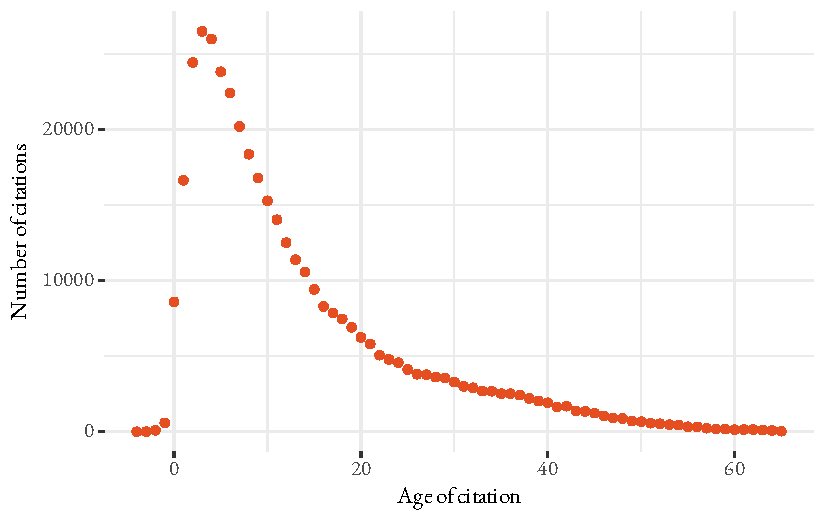
\includegraphics[keepaspectratio]{apc-2025_files/figure-pdf/fig-overall-age-1.pdf}}

}

\caption{\label{fig-overall-age}Number of citations with each age.}

\end{figure}%

In Figure~\ref{fig-overall-median-mode} I've plotted the median and mode
age of citations in each year from 1980 onwards. Before that the numbers
are even lower, but since I'm only looking at citations to articles
published after 1955 (or later if Web of Science started indexing the
journal later than that), this is arguably an artifact of how I'm
collecting the data. From 1980 onwards, however, there are many older
articles that could be, but are not, getting cited. The upwards trends
in both graphs look like a real change in citation practices, and not in
the direction I antecedently expected.

\begin{figure}

\begin{minipage}{\linewidth}

\centering{

\pandocbounded{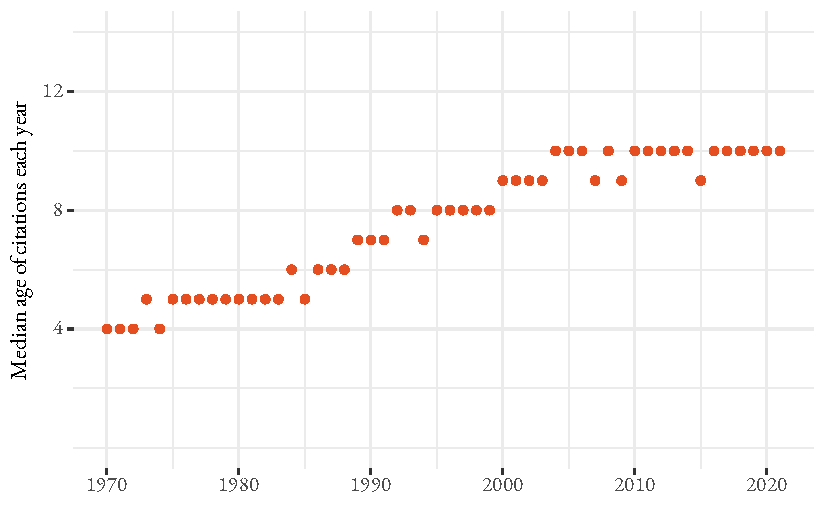
\includegraphics[keepaspectratio]{apc-2025_files/figure-pdf/fig-overall-median-mode-1.pdf}}

}

\subcaption{\label{fig-overall-median-mode-1}Median}

\end{minipage}%
\newline
\begin{minipage}{\linewidth}

\centering{

\pandocbounded{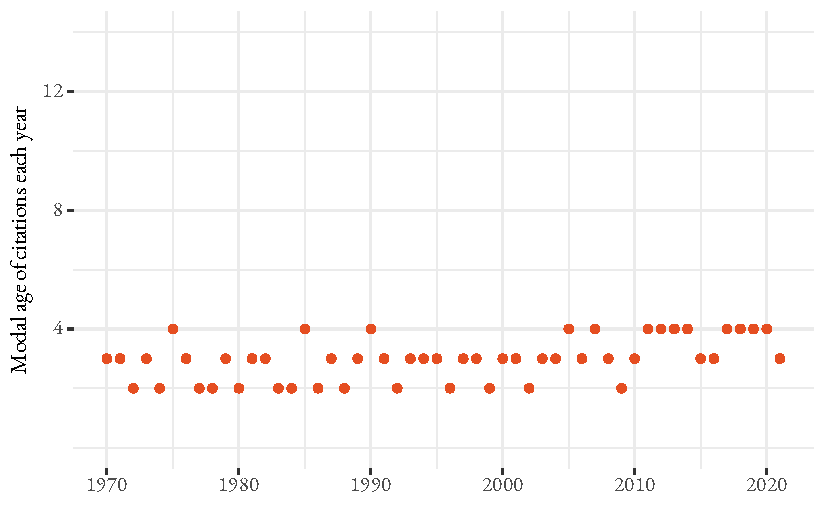
\includegraphics[keepaspectratio]{apc-2025_files/figure-pdf/fig-overall-median-mode-2.pdf}}

}

\subcaption{\label{fig-overall-median-mode-2}Mode}

\end{minipage}%

\caption{\label{fig-overall-median-mode}Summary statistics for outbound
citations each year 1970-2021.}

\end{figure}%

There is a third surprise in the data, but it's a little more equivocal,
and I'm not sure what to make of it. The 2010s seemed like, and to be
honest still seem like, something of a golden age for philosophy. In
metaphysics we saw the biggest paradigm shift in many years, away from
modality and towards grounding. We saw the growth of important fields of
social philosophy, including social epistemology, social metaphysics,
and social philosophy of language. Though there were some earlier papers
that have become important to the latter two fields (e.g., Haslanger
(\citeproc{ref-Haslanger2000}{2000a}), and Langton
(\citeproc{ref-Langton1993}{1993})), it would have been a stretch to
even call them `fields' before 2010. Social epistemology was always a
bit bigger, and you could point to earlier field defining work by, e.g.,
Jennifer Lackey (\citeproc{ref-Lackey2008}{2008}) and Adam Elga
(\citeproc{ref-Elga2007}{2007a}). But it grew phenomenally in the 2010s.
I'd predicted that would show up in higher citations to work in the
2010s, as these changes were consolidated. The data are a bit messy, and
it would be good to have much more data, but this does not look to have
happened. There isn't as neat a graph for this, however, and we'll
return to this point at the end.

\section{Age, Period, and Cohort}\label{sec-apc-described}

To help understand the citation patterns, I'll borrow some terminology
that's common in both sociology and medicine. Imagine that we see, in
the historical record, some interesting patterns among teenagers in the
late 1960s, and we're wondering what could explain the pattern. Two
types of pattern spring immediately to mind, along with ways to test
them.

First, the behaviour could be explained by the fact the people involved
are teenagers. If so, it is an \textbf{age effect}. The natural way to
test this is to see if similar patterns show up with teenagers at
different times.

Second, the behaviour could be explained by the fact that it was the
1960s, and lots of striking things happened in the 1960s. If so, it is a
\textbf{period effect}. The natural way to test this is to see if the
same pattern shows up with non-teenagers in the 1960s.

There is an important third kind of explanation. The people involved are
born in the early 1950s, so they are part of the post-war baby boom.
Colloquially, they are boomers. Maybe that could explain the pattern we
see. If so, it is a \textbf{cohort effect}. The natural way to test this
is to see if the same pattern shows up if we look at the same people in
other stages of their life.

It's easy to overlook the importance of cohort effects. Sometimes they
simply look like age effects. Ghitza, Gelman, and Auerbach
(\citeproc{ref-GhitzaEtAl2023}{2023}) argue that many hypotheses about
age effects on voting, e.g., that older people are more naturally
conservative, are really just cohort effects. Bump
(\citeproc{ref-Bump2023}{2023}) argues that understanding the
distinctive role the boomers in particular play is crucial for
understanding many aspects of modern American life.

There are mathematical reasons that it is hard to tease these effects
apart too. Many statistical techniques for separating out influences
start to fall apart when there are linear correlations between
combinations of variables. In this case there is as tight a correlation
as is possible. By definition, cohort plus age equals period. There are
some things you can do to get around this problem - see Keyes et al.
(\citeproc{ref-KeyesEtAl2010}{2010}) for a useful survey of some of the
options - but it remains a challenge.

Even conceptually, it is hard to separate out these three effects in
cases where there is evidence that the strength of the effects changes
over time. As I noted at the start, the natural way to test hypotheses
about which effect is strongest involve looking at other times. That
works well when the age effects are constant. When they are not (and
they might not be here), it is harder.

For most of our story, however, it helps just to have these three
effects in mind. Using them, we can summarise the data reasonably
quickly.

\begin{itemize}
\tightlist
\item
  The age effect is that articles get cited most when they are two to
  five years old, as shown in Figure~\ref{fig-overall-age}.
\item
  The period effect is that there are many more citations in recent
  years than in earlier years. This is in part because the number of
  articles published in these journals has been growing, and in part
  because the number of citations per article grew substantially over
  the 2000s and 2010s, and exploded in the 2020s.
\item
  The cohort effect is that articles from the 1970s and 2000s get cited
  more than you'd expect given these age and period effects, articles
  from before the late-1960s get barely cited at all, and articles from
  1980 through the mid-1990s also get cited considerably less than
  articles either side of that period. I'll offer some speculations at
  the end of the paper about the philosophical causes of, and
  consequences of, these cohort effects.
\end{itemize}

As I mentioned above, I'll go over the methodology in detail in
\textbf{?@sec-methodology}. But there is one point that is important to
note before we start. I'm using data from Web of Science, and they
typically don't start indexing journals until well after the journal is
established. So the first year of citation data I have for
\emph{Analysis} is 1975. Crucially, that means that ``Is Knowledge
Justified True Belief?'' (\citeproc{ref-Gettier1963}{Gettier 1963}) is
not included in this study. If it were, and in general if I had the data
from \emph{Analysis} to work from, some of the results about the early
1960s would look less dramatic, though as far as I can tell, the
direction of the results wouldn't change.

\section{Period Effects}\label{sec-period}

Those 397368 citations are not distributed evenly over time. Instead,
they grow rapidly. At the start, in 1956, there are only 5 citations.
That's not too surprising; without the ability to cite preprints, there
aren't going to be many citations of articles that have come out that
year. By 2021, there are 56293. In Figure~\ref{fig-citationsperyear}, I
show how these grew; the striking thing to me is the big jump between
2020 and 2021.

\begin{figure}

\centering{

\pandocbounded{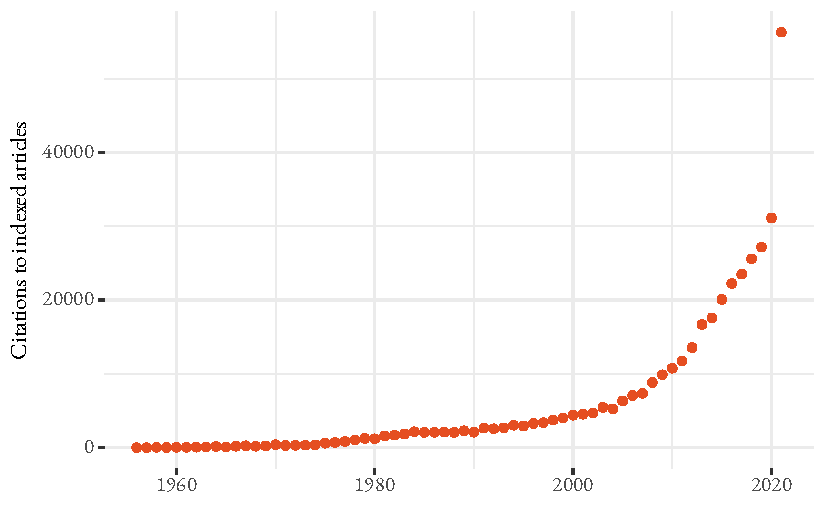
\includegraphics[keepaspectratio]{apc-2025_files/figure-pdf/fig-citationsperyear-1.pdf}}

}

\caption{\label{fig-citationsperyear}The number of citations in the
dataset made each year.}

\end{figure}%

What explains this dramatic growth? Part of the explanation is that more
articles are being published, and more articles are being indexed.
Figure~\ref{fig-articlesperyear} shows how many articles are in the
dataset each year.

\begin{figure}

\centering{

\pandocbounded{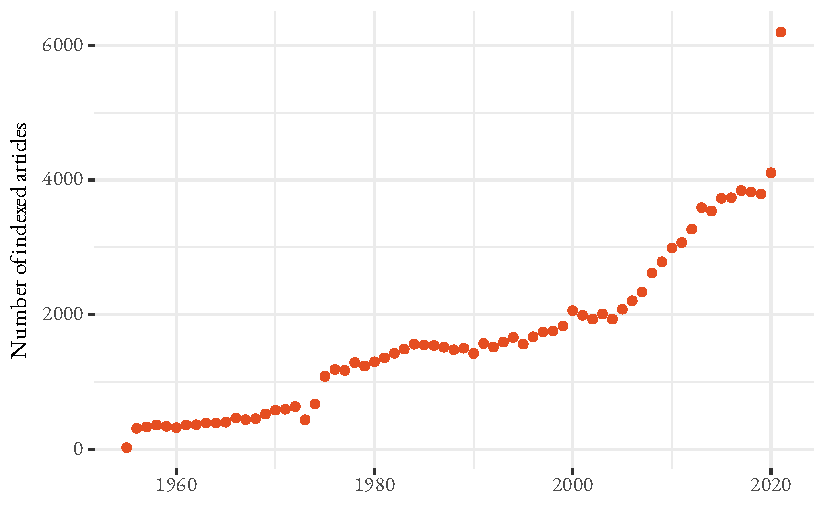
\includegraphics[keepaspectratio]{apc-2025_files/figure-pdf/fig-articlesperyear-1.pdf}}

}

\caption{\label{fig-articlesperyear}The number of articles in the
dataset published each year.}

\end{figure}%

That explains some of the growth, but not all of it. The curve in
Figure~\ref{fig-articlesperyear} is not nearly as steep as the curve in
Figure~\ref{fig-citationsperyear}. The number of (indexed) citations per
article is also rising. In Figure~\ref{fig-outboundcitations} I've
plotted the average number of citations to other articles in the dataset
each year.

\begin{figure}

\centering{

\pandocbounded{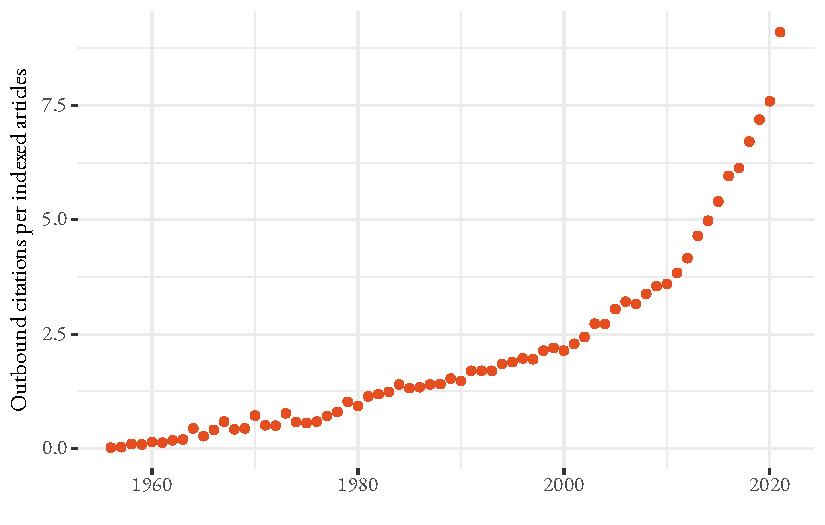
\includegraphics[keepaspectratio]{apc-2025_files/figure-pdf/fig-outboundcitations-1.pdf}}

}

\caption{\label{fig-outboundcitations}The average number of citations to
indexed articles each year.}

\end{figure}%

There are a few possible explanations for the shape of this graph.

At the left-hand edge, there are obvious boundary effects. Since we're
only counting citations to articles published since 1956, it isn't
surprising that there aren't very many of them per article in the 1950s.
Since articles rarely get unpublished, there are more articles available
to cite every year.

That can't explain the massive jumps we see at the right hand edge of
Figure~\ref{fig-outboundcitations}. The jump there looks like the
convergence of two cultural trends. One is a trend simply to greater
numbers of citations. The most casual perusal of journals will confirm
that trend. The other is a trend to greater citations of journals
themselves, as opposed to books or edited volumes.

A sharp jump like this is a warning sign that there is something wrong
with the data. It's impractical to cross-check every entry, but those I
have checked look correct. The change seems led by the most prestigious
journals. For each journal I calculated the average number of outbound
citations (to these hundred journal) for both the 2010s, and the first
two years of the 2020s. The ten journals with the largest increase
between the decades are shown in Table~\ref{tbl-large-growth}.

\begin{longtable}[]{@{}
  >{\raggedright\arraybackslash}p{(\linewidth - 6\tabcolsep) * \real{0.5694}}
  >{\raggedleft\arraybackslash}p{(\linewidth - 6\tabcolsep) * \real{0.1389}}
  >{\raggedleft\arraybackslash}p{(\linewidth - 6\tabcolsep) * \real{0.1389}}
  >{\raggedleft\arraybackslash}p{(\linewidth - 6\tabcolsep) * \real{0.1528}}@{}}

\caption{\label{tbl-large-growth}Mean outbound citations for some
journals over the last two decades.}

\tabularnewline

\toprule\noalign{}
\begin{minipage}[b]{\linewidth}\raggedright
Journal
\end{minipage} & \begin{minipage}[b]{\linewidth}\raggedleft
2010-2019
\end{minipage} & \begin{minipage}[b]{\linewidth}\raggedleft
2020-2021
\end{minipage} & \begin{minipage}[b]{\linewidth}\raggedleft
Difference
\end{minipage} \\
\midrule\noalign{}
\endhead
\bottomrule\noalign{}
\endlastfoot
Philosophical Review & 14.8 & 26.3 & 11.5 \\
Philosophical Perspectives & 11.3 & 19.6 & 8.3 \\
Philosophy and Phenomenological Research & 9.6 & 15.2 & 5.6 \\
Journal of Philosophy & 9.0 & 13.7 & 4.8 \\
Philosophical Studies & 9.0 & 13.6 & 4.6 \\
Noûs & 11.5 & 16.0 & 4.5 \\
Philosophical Quarterly & 8.8 & 13.3 & 4.5 \\
Philosophy & 4.0 & 8.3 & 4.3 \\
Philosophy Compass & 11.2 & 15.4 & 4.3 \\
Philosophia Mathematica & 6.3 & 10.1 & 3.8 \\

\end{longtable}

Since \emph{Philosophical Review} only publishes 10 to 12 articles per
year, it is not surprising that it shows the most variation on this
list. Still, the change in the 2010s isn't only small sample size
variation. Of the 22 articles it published in 2020 and 2021, only one of
them (\citeproc{ref-WOS000575210400003}{Oberman 2020}) had fewer than
14.8 outbound citations. With a sample of just 22 anything could happen,
but it would be surprising to have all but one end up on the same side
of the historical average by chance.

Although the number of citations is going up, the number of articles
available to be cited is also going up. Say an article is
\emph{available} if it is published in a year iff it is published in or
before that year. That's not quite right in either direction; some
articles are cited before publication, some articles that come out in
December aren't in any real sense available to be cited in January. But
it's close enough. Say an article is from a year that is
\emph{typically} cited iff it is between 3 and 10 years before the
citing year. This notion will play a big role in \textbf{?@sec-age}; I'm
going to use these as a way of getting something like a base rate for
citations in a given year. Using these definitions,
Figure~\ref{fig-articlecounts} shows how many articles are available to
be cited each year, and are from years that are typically cited.

\begin{figure}

\begin{minipage}{\linewidth}

\centering{

\pandocbounded{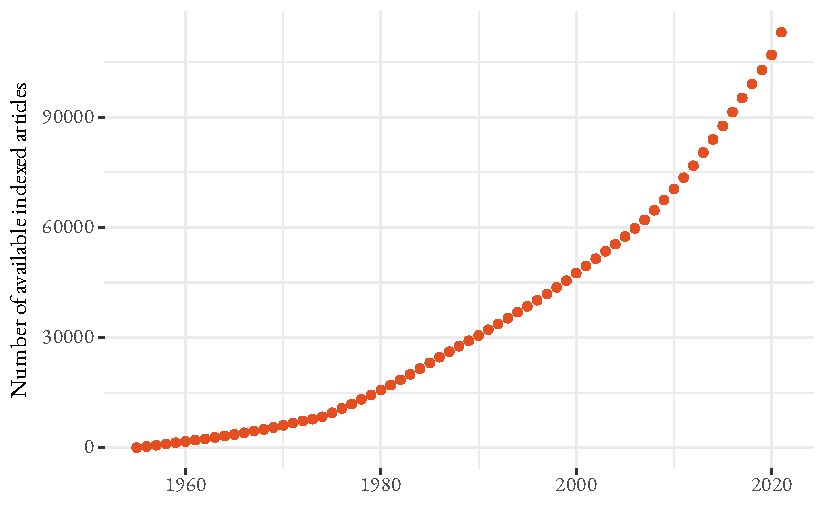
\includegraphics[keepaspectratio]{apc-2025_files/figure-pdf/fig-articlecounts-1.pdf}}

}

\subcaption{\label{fig-articlecounts-1}Available articles}

\end{minipage}%
\newline
\begin{minipage}{\linewidth}

\centering{

\pandocbounded{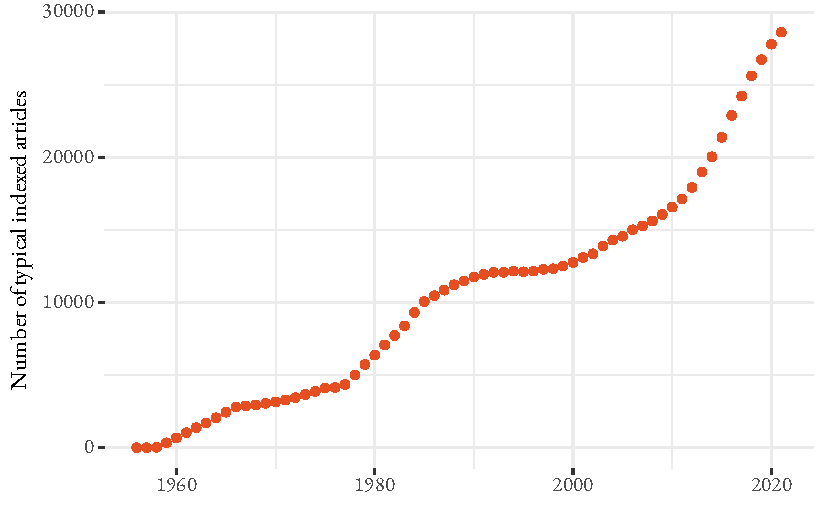
\includegraphics[keepaspectratio]{apc-2025_files/figure-pdf/fig-articlecounts-2.pdf}}

}

\subcaption{\label{fig-articlecounts-2}Typically cited articles}

\end{minipage}%

\caption{\label{fig-articlecounts}Article counts.}

\end{figure}%

In Figure~\ref{fig-citationcounts}, I've shown how often, in each year,
the available articles, and the `typical' articles are cited. The
`available' graph is obviously similar to
Figure~\ref{fig-citationsperyear}; under 1\% of citations are to
articles published in future years. One thing that will be useful in
\textbf{?@sec-age} is that the graphs in Figure~\ref{fig-citationcounts}
have a similar shape.

\begin{figure}

\begin{minipage}{\linewidth}

\centering{

\pandocbounded{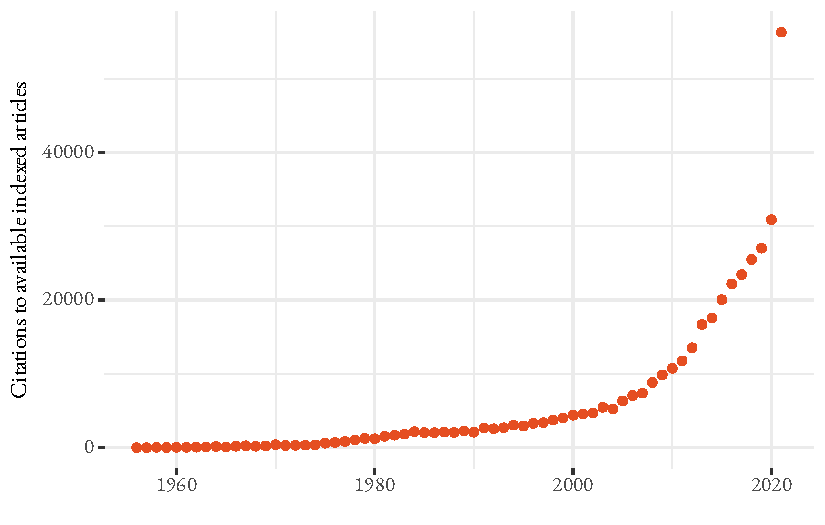
\includegraphics[keepaspectratio]{apc-2025_files/figure-pdf/fig-citationcounts-1.pdf}}

}

\subcaption{\label{fig-citationcounts-1}Citations to available articles}

\end{minipage}%
\newline
\begin{minipage}{\linewidth}

\centering{

\pandocbounded{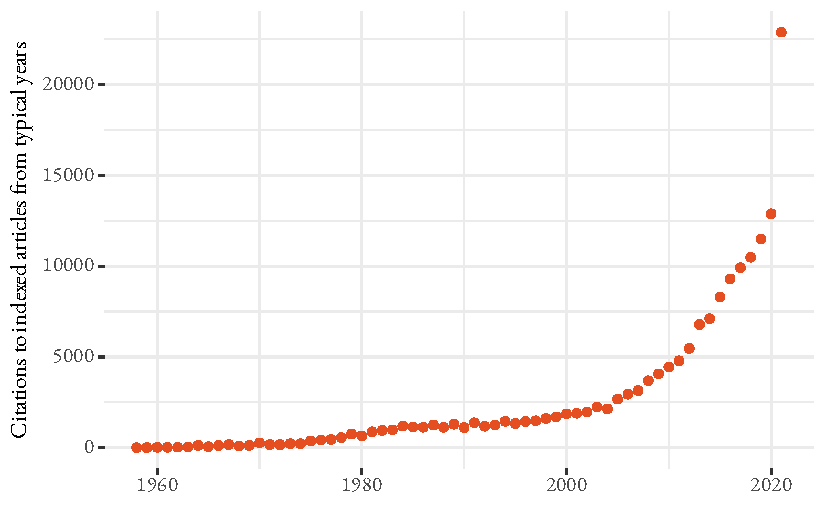
\includegraphics[keepaspectratio]{apc-2025_files/figure-pdf/fig-citationcounts-2.pdf}}

}

\subcaption{\label{fig-citationcounts-2}Citations to typical articles}

\end{minipage}%

\caption{\label{fig-citationcounts}Citation counts.}

\end{figure}%

Putting all these together we can work out how often, on average,
available articles, and typical articles, are cited in each year. The
results are in Figure~\ref{fig-citationrate}.

\begin{figure}

\begin{minipage}{\linewidth}

\centering{

\pandocbounded{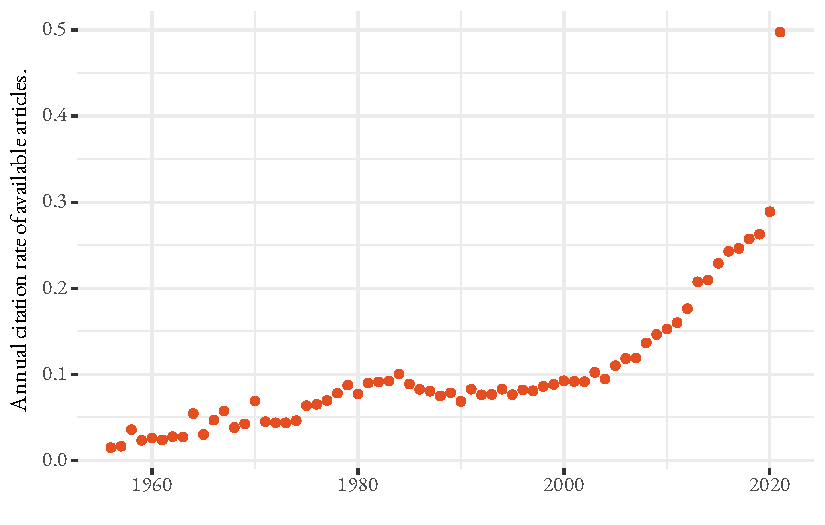
\includegraphics[keepaspectratio]{apc-2025_files/figure-pdf/fig-citationrate-1.pdf}}

}

\subcaption{\label{fig-citationrate-1}Available articles}

\end{minipage}%
\newline
\begin{minipage}{\linewidth}

\centering{

\pandocbounded{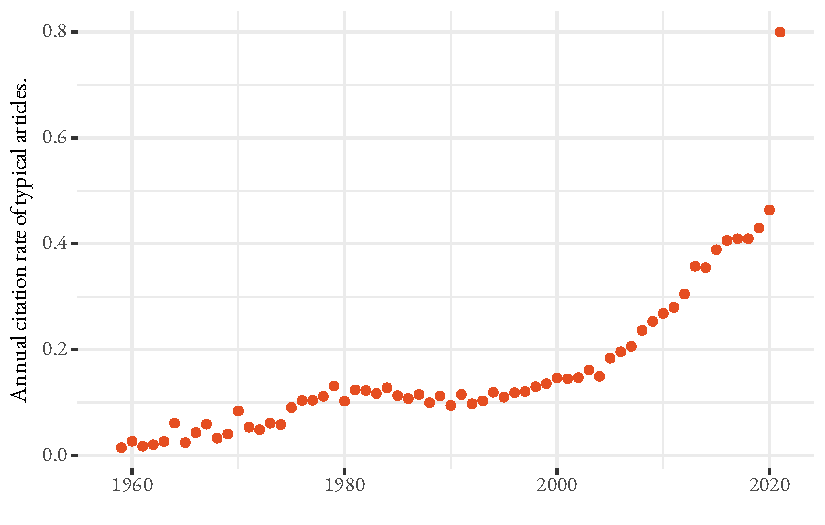
\includegraphics[keepaspectratio]{apc-2025_files/figure-pdf/fig-citationrate-2.pdf}}

}

\subcaption{\label{fig-citationrate-2}Typical articles}

\end{minipage}%

\caption{\label{fig-citationrate}Mean annual citations to different
article kinds.}

\end{figure}%

Three things stand out about Figure~\ref{fig-citationrate}. One is that
the two graphs have pretty similar shapes. Using citations from 3 to 10
years prior to the citing year is a pretty good proxy for all citations,
and it turns out to be stable in other ways. A second is that both
graphs are fairly flat for a long time. Between the mid 1970s and early
2000s they bounce around without moving much. Then they take off, and go
through the roof in 2021. The other thing is that these are low numbers.
For most of this study, an arbitrary article in one of these hundred
journals was cited in one of those journals once a \emph{decade}.
Actually, since citation rates are extremely long-tailed, and mean rates
are well above medians, that somewhat overstates how often the `average
article' was being cited. Frequent citation is very much not the
norm.\footnote{In the long run the average number of times an article is
  cited equals the average number of citations per article. So it
  shouldn't be too surprising that most article have just a handful of
  citations in philosophy journals.}

The various period effects are substantial; to get an reliable picture
of the trends in citation patterns, we're going to have to allow for
them. The project here is to use citation data as a proxy for
philosophical influence. It is, of course, a deeply imperfect proxy. But
it is better than most other proxies; it is certainly better than going
off of vibes, or of what one's friends are talking about.\footnote{In
  North America, placement on graduate syllabi might be an even better
  proxy, but that data is hard to collect, and we'd need a different
  measure for other countries.} If we're going to use citations this way
though, we need to think about how to take into account the changes
shown in Figure~\ref{fig-citationsperyear}. I'm going to offer a
proposal in terms of typical articles; to a first approximation, I'll
measure an article's influence in a period by the ratio of how often it
is cited to how often a typical article is cited. This is a little
arbitrary, but I think it gets things at least roughly right. At the
very least, it avoids the problems with three other natural proposals
that I'll now present, and probably anything that avoids these problems
will be fairly similar.

Start with the non-proposal of just using citations per year as a
measure of influence. Simply eyeballing
Figure~\ref{fig-citationsperyear} makes that a little implausible; there
would be so much more influence now. It also has some implausible
particular consequences. Tyler Burge's ``Individualism and Psychology''
(\citeproc{ref-WOSA1986AYX3200001}{Burge 1986}) was the fourth most
cited paper of the 1990s, and if anything that understates its
influence. In the 1990s (in these 100 journals) it had 68 citations, so
6.8 per year. In 2021, it had 7 citations, so slightly more per year.
Now Burge's paper is still influential, and it connects in interesting
ways to the social turn in philosophy that I'll discuss below, but it's
implausible to say that it was more influential in 2021 than it was in
the 1990s. When there are so many articles published, and a much lower
bar to citation, seven citations a year doesn't signify as much
influence.

A natural second proposal then is to measure what proportion of the
year's citations any particular article has. By this measure,
``Individualism and Psychology'' was about twenty times as influential
in the 1990s as in 2021, which isn't obviously false.\footnote{To be
  clear, the database contains about twice as many citations in 2021 as
  in the whole of the 1990s.} Other cases, however, suggest this is too
much of a correction. It's true that there are more citations now than
there used to be. There are also more articles for these citations to be
shared between. Holding fixed how influential an article is, you'd
expect it to have a lower share of the citations when there are several
times more articles available to be cited.

Again, it's easiest to see this with some examples. In
Table~\ref{tbl-comp-cite-rate}, I've shown the five most cited articles
for the 1990s (on the top), and for 2021 (on the bottom). I've also
shown how often each is cited per 1000 citations, i.e., the proportion
of citations each article gets. And I've extended the first table to
make it easier to compare the scales.

\begin{table}

\caption{\label{tbl-comp-cite-rate}Most cited articles in the 1990s, and
in 2021.}

\begin{minipage}{\linewidth}

\subcaption{\label{tbl-comp-cite-rate-1}1990s}

\centering{

\begin{tabular}{rlrr}
\toprule
Rank & Article & Citations & Citations per 1000\\
\midrule
1 & Frankfurt (\citeproc{ref-10.2307_2024717}{1971}) & 82 & 2.69\\
2 & Kim (\citeproc{ref-WOSA1984TV24600001}{1984}) & 72 & 2.36\\
3 & Nagel (\citeproc{ref-WOSA1974U469700001}{1974}) & 69 & 2.27\\
4 & Burge (\citeproc{ref-WOSA1986AYX3200001}{1986}) & 68 & 2.23\\
 & \ldots{} &  & \\
10 & Kripke (\citeproc{ref-WOSA1975BF60000005}{1975}) & 52 & 1.71\\
 & \ldots{} &  & \\
34 & Hull (\citeproc{ref-WOSA1978FR68900001}{1978}) & 33 & 1.08\\
35 & Lewis (\citeproc{ref-WOSA1979JB14500003}{1979}) & 33 & 1.08\\
36 & Fraassen (\citeproc{ref-WOSA1984SS95000001}{1984}) & 33 & 1.08\\
\bottomrule
\end{tabular}

}

\end{minipage}%
\newline
\begin{minipage}{\linewidth}

\subcaption{\label{tbl-comp-cite-rate-2}2021}

\centering{

\begin{tabular}{rlrr}
\toprule
Rank & Article & Citations & Citations per 1000\\
\midrule
1 & Lewis (\citeproc{ref-WOSA1983RR51600001}{1983}) & 96 & 1.71\\
2 & Haslanger (\citeproc{ref-WOS000085841900002}{2000b}) & 60 & 1.07\\
3 & Machamer, Darden, and Craver
(\citeproc{ref-WOS000087305900001}{2000}) & 56 & 0.99\\
4 & Clark and Chalmers
(\citeproc{ref-WOS000073222300002}{1998}) & 54 & 0.96\\
5 & Schaffer (\citeproc{ref-WOS000272855000002}{2010}) & 54 & 0.96\\
6 & Elga (\citeproc{ref-WOS000249103800005}{2007b}) & 52 & 0.92\\
7 & Lewis (\citeproc{ref-10.2307_2025310}{1973b}) & 51 & 0.91\\
8 & Christensen (\citeproc{ref-WOS000207419300002}{2007}) & 50 & 0.89\\
9 & Schaffer (\citeproc{ref-WOS000368189400004}{2016}) & 46 & 0.82\\
10 & Nagel (\citeproc{ref-WOSA1974U469700001}{1974}) & 46 & 0.82\\
\bottomrule
\end{tabular}

}

\end{minipage}%

\end{table}%

As influential as ``A Matter of Individuality'', ``Counterfactual
Dependence and Time's Arrow'', and ``Belief and the Will'' were in the
1990s, I don't think they were more influential than all but one article
was in 2021. Haslanger's article became a foundational text for one of
the biggest fields in philosophy: social metaphysics. A measure of
influence that puts it behind how influential 36 articles were in the
1990s seems wrong, and the intuitive reasoning about sharing citations
around suggests why it is wrong.

A natural next move is to scale the citations not to all citations, but
to the average number of citations that available, i.e., already
published, articles get. This would solve the problem I just presented
in a simple way. Having 1 cite per 1000 citations means a lot more when
there are 100,000 articles that could have received that citation than
when there are 10,000 such articles.

Again, this is an overcorrection. In theory, any article already
published could be cited. In practice, long forgotten articles are long
forgotten and hence not cited, and most articles are long forgotten.
It's true that in 2021 articles have to `share' citation space with more
other articles. But in practice that normally means they share the space
with other \emph{recently published} articles.

We can sort of see this by redoing the calculation from
Table~\ref{tbl-comp-cite-rate}, instead using the ratio of citations
this article receives to citations the average available article
receives.\footnote{On the first part of Table~\ref{tbl-comp-cite-ratio},
  I calculated this ratio for each year, and then displayed the average
  over the decade.} I've done this in Table~\ref{tbl-comp-cite-ratio}.
First, I've shown the articles that, across the 1990s, had the highest
average ratio of citations they received to citations the average
available article received, and second, I did the same calculation for
2021.

\begin{table}

\caption{\label{tbl-comp-cite-ratio}Most cited articles in the 1990s
compared to average citations, and in 2021.}

\begin{minipage}{\linewidth}

\subcaption{\label{tbl-comp-cite-ratio-1}1990s}

\centering{

\begin{tabular}{rlr}
\toprule
Rank & Article & Ratio\\
\midrule
1 & Frankfurt (\citeproc{ref-10.2307_2024717}{1971}) & 102.45\\
2 & Kim (\citeproc{ref-WOSA1984TV24600001}{1984}) & 90.15\\
3 & Nagel (\citeproc{ref-WOSA1974U469700001}{1974}) & 85.95\\
4 & Burge (\citeproc{ref-WOSA1986AYX3200001}{1986}) & 85.05\\
5 & Perry (\citeproc{ref-WOSA1979HE39600001}{1979}) & 78.28\\
6 & Lewis (\citeproc{ref-WOSA1983RR51600001}{1983}) & 76.01\\
7 & Jackson (\citeproc{ref-WOSA1982NH65300003}{1982}) & 71.51\\
8 & Kripke (\citeproc{ref-WOSA1975BF60000005}{1975}) & 65.91\\
9 & Cummins (\citeproc{ref-WOSA1975BF60100001}{1975}) & 65.29\\
10 & Lewis (\citeproc{ref-10.2307_2025310}{1973b}) & 64.95\\
\bottomrule
\end{tabular}

}

\end{minipage}%
\newline
\begin{minipage}{\linewidth}

\subcaption{\label{tbl-comp-cite-ratio-2}2021}

\centering{

\begin{tabular}{rlr}
\toprule
Rank & Article & Ratio\\
\midrule
1 & Lewis (\citeproc{ref-WOSA1983RR51600001}{1983}) & 192.98\\
2 & Haslanger (\citeproc{ref-WOS000085841900002}{2000b}) & 120.61\\
3 & Machamer, Darden, and Craver
(\citeproc{ref-WOS000087305900001}{2000}) & 112.57\\
4 & Clark and Chalmers
(\citeproc{ref-WOS000073222300002}{1998}) & 108.55\\
5 & Schaffer (\citeproc{ref-WOS000272855000002}{2010}) & 108.55\\
6 & Elga (\citeproc{ref-WOS000249103800005}{2007b}) & 104.53\\
 & \ldots{} & \\
12 & Plunkett and Sundell
(\citeproc{ref-WOS000332023600001}{2013}) & 90.46\\
 & \ldots{} & \\
35 & Dorr (\citeproc{ref-WOS000397575900003}{2016}) & 66.34\\
\bottomrule
\end{tabular}

}

\end{minipage}%

\end{table}%

None of the pairwise comparisons here seem obviously absurd. Was ``To be
F is to be G'' more influential in 2021 than ``Causation'' was in the
1990s? I wouldn't have thought so, but it's not as clear as in the
previous set of comparisons. But it is clear that the numbers in the
second table in Table~\ref{tbl-comp-cite-ratio} are considerably higher
than the first table, especially at the very top end. That suggests that
the intuition that including so many articles from long ago in the
comparison class was a mistake, and it has systematically increased the
measure we're using for later years in implausible ways.

So what I've settled on is using the ratio of how often this article is
cited in a year, to how often a \emph{typical} article is cited that
year. By `typical' I mean an article three to ten years old; as we'll
see in \textbf{?@sec-age}, those are the typical ages of cited articles.
That deals with the intuitive problems of the previous measures, and it
gets the results roughly right. In
Table~\ref{tbl-comp-cite-ratio-typical}, I'll do one last comparison
between the 1990s and 2021 to make the point.

\begin{table}

\caption{\label{tbl-comp-cite-ratio-typical}Most cited articles in the
1990s compared to typical citations, and in 2021.}

\begin{minipage}{\linewidth}

\subcaption{\label{tbl-comp-cite-ratio-typical-1}1990s}

\centering{

\begin{tabular}{rlr}
\toprule
Rank & Article & Ratio\\
\midrule
1 & Frankfurt (\citeproc{ref-10.2307_2024717}{1971}) & 71.87\\
2 & Kim (\citeproc{ref-WOSA1984TV24600001}{1984}) & 63.99\\
3 & Nagel (\citeproc{ref-WOSA1974U469700001}{1974}) & 60.03\\
4 & Burge (\citeproc{ref-WOSA1986AYX3200001}{1986}) & 59.88\\
5 & Perry (\citeproc{ref-WOSA1979HE39600001}{1979}) & 55.46\\
6 & Lewis (\citeproc{ref-WOSA1983RR51600001}{1983}) & 53.21\\
7 & Jackson (\citeproc{ref-WOSA1982NH65300003}{1982}) & 49.90\\
8 & Kripke (\citeproc{ref-WOSA1975BF60000005}{1975}) & 46.45\\
9 & Churchland (\citeproc{ref-WOSA1981LD54600001}{1981}) & 45.63\\
10 & Lewis (\citeproc{ref-10.2307_2025310}{1973b}) & 45.25\\
\bottomrule
\end{tabular}

}

\end{minipage}%
\newline
\begin{minipage}{\linewidth}

\subcaption{\label{tbl-comp-cite-ratio-typical-2}2021}

\centering{

\begin{tabular}{rlr}
\toprule
Rank & Article & Ratio\\
\midrule
1 & Lewis (\citeproc{ref-WOSA1983RR51600001}{1983}) & 120.04\\
2 & Haslanger (\citeproc{ref-WOS000085841900002}{2000b}) & 75.02\\
3 & Machamer, Darden, and Craver
(\citeproc{ref-WOS000087305900001}{2000}) & 70.02\\
4 & Clark and Chalmers
(\citeproc{ref-WOS000073222300002}{1998}) & 67.52\\
5 & Schaffer (\citeproc{ref-WOS000272855000002}{2010}) & 67.52\\
6 & Elga (\citeproc{ref-WOS000249103800005}{2007b}) & 65.02\\
7 & Lewis (\citeproc{ref-10.2307_2025310}{1973b}) & 63.77\\
8 & Christensen (\citeproc{ref-WOS000207419300002}{2007}) & 62.52\\
9 & Schaffer (\citeproc{ref-WOS000368189400004}{2016}) & 57.52\\
10 & Nagel (\citeproc{ref-WOSA1974U469700001}{1974}) & 57.52\\
\bottomrule
\end{tabular}

}

\end{minipage}%

\end{table}%

The numbers in the second table are a little higher, but not overly so.
In any case, one would expect the top end of a scale like this to be
higher when just looking at a single year, where there is more
variation, than at an average over a decade.\footnote{If I did the same
  comparison year-by-year, there are individual years where ``Meaning''
  (\citeproc{ref-WOSA1957CGZ6000005}{Grice 1957}), ``Justice as
  Fairness: Political not Metaphysical''
  (\citeproc{ref-WOSA1985APA8500001}{Rawls 1985}) and ``Concepts of
  Supervenience'' (\citeproc{ref-WOSA1984TV24600001}{Kim 1984}) have a
  higher ratio of citations to the average typical article than ``New
  Work'' does in 2021.} So I'll take this as the measure of age-adjusted
number of citations. That is, to factor out the age effect on citations,
I'll divide the number of citations an article receives in a year by the
average number that a typical, i.e., 3-10 year old, article receives
that year.

\phantomsection\label{refs}
\begin{CSLReferences}{1}{0}
\bibitem[\citeproctext]{ref-Bump2023}
Bump, Philip. 2023. \emph{The Aftermath: The Last Days of the Baby Boom
and the Future of Power in America}. New York: Penguin Random House.

\bibitem[\citeproctext]{ref-WOSA1986AYX3200001}
Burge, Tyler. 1986. {``Individualism and Psychology.''}
\emph{Philosophical Review} 95 (1): 3--45.
\url{https://doi.org/10.2307/2185131}.

\bibitem[\citeproctext]{ref-WOS000207419300002}
Christensen, David. 2007. {``Epistemology of Disagreement: The Good
News.''} \emph{Philosophical Review} 116 (2): 187--217.
\url{https://doi.org/10.1215/00318108-2006-035}.

\bibitem[\citeproctext]{ref-WOSA1981LD54600001}
Churchland, Paul M. 1981. {``Eliminative Materialism and the
Propositional Attitudes.''} \emph{Journal of Philosophy} 78 (2): 67--90.
\url{https://doi.org/10.2307/2025900}.

\bibitem[\citeproctext]{ref-WOS000073222300002}
Clark, Andy, and David J. Chalmers. 1998. {``The Extended Mind.''}
\emph{Analysis} 58 (1): 7--19.
\url{https://doi.org/10.1111/1467-8284.00096}.

\bibitem[\citeproctext]{ref-WOSA1975BF60100001}
Cummins, Robert. 1975. {``Functional Analysis.''} \emph{Journal of
Philosophy} 72 (20): 741--65. \url{https://doi.org/10.2307/2024640}.

\bibitem[\citeproctext]{ref-WOS000397575900003}
Dorr, Cian. 2016. {``To Be f Is to Be g.''} \emph{Philosophical
Perspectives} 30 (1): 39--134. \url{https://doi.org/10.1111/phpe.12079}.

\bibitem[\citeproctext]{ref-Elga2007}
Elga, Adam. 2007a. {``Reflection and Disagreement.''} \emph{No{û}s} 41
(3): 478--502. \url{https://doi.org/10.1111/j.1468-0068.2007.00656.x}.

\bibitem[\citeproctext]{ref-WOS000249103800005}
---------. 2007b. {``Reflection and Disagreement.''} \emph{Noûs} 41 (3):
478--502. \url{https://doi.org/10.1111/j.1468-0068.2007.00656.x}.

\bibitem[\citeproctext]{ref-WOSA1984SS95000001}
Fraassen, Bas C. van. 1984. {``Belief and the Will.''} \emph{Journal of
Philosophy} 81 (5): 235--56.

\bibitem[\citeproctext]{ref-Frankfurt1969}
Frankfurt, Harry G. 1969. {``Alternate Possibilities and Moral
Responsibility.''} \emph{Journal Of Philosophy} 66 (23): 829--39.
\url{https://doi.org/10.2307/2023833}.

\bibitem[\citeproctext]{ref-10.2307_2024717}
---------. 1971. {``Freedom of the Will and the Concept of a Person.''}
\emph{Journal of Philosophy} 68 (1): 5--20.

\bibitem[\citeproctext]{ref-Gettier1963}
Gettier, Edmund L. 1963. {``Is Justified True Belief Knowledge?''}
\emph{Analysis} 23 (6): 121--23. \url{https://doi.org/10.2307/3326922}.

\bibitem[\citeproctext]{ref-GhitzaEtAl2023}
Ghitza, Yair, Andrew Gelman, and Jonathan Auerbach. 2023. {``The Great
Society, Reagan's Revolution, and Generations of Presidential Voting.''}
\emph{American Journal of Political Science} 67 (3): 520--37.
https://doi.org/\url{https://doi.org/10.1111/ajps.12713}.

\bibitem[\citeproctext]{ref-WOSA1957CGZ6000005}
Grice, H. P. 1957. {``Meaning.''} \emph{Philosophical Review} 66 (3):
377--88. \url{https://doi.org/10.2307/2182440}.

\bibitem[\citeproctext]{ref-Haslanger2000}
Haslanger, Sally. 2000a. {``Gender and Race: (What) Are They? (What) Do
We Want Them to Be?''} \emph{No{û}s} 34 (1): 31--55.
\url{https://doi.org/10.1111/0029-4624.00201}.

\bibitem[\citeproctext]{ref-WOS000085841900002}
---------. 2000b. {``Gender and Race: (What) Are They? (What) Do We Want
Them to Be?''} \emph{Noûs} 34 (1): 31--55.
\url{https://doi.org/10.1111/0029-4624.00201}.

\bibitem[\citeproctext]{ref-WOSA1978FR68900001}
Hull, David L. 1978. {``A Matter of Individuality.''} \emph{Philosophy
of Science} 45 (3): 335--60. \url{https://doi.org/10.1086/288811}.

\bibitem[\citeproctext]{ref-WOSA1982NH65300003}
Jackson, Frank. 1982. {``Epiphenomenal Qualia.''} \emph{Philosophical
Quarterly} 32 (127): 127--36. \url{https://doi.org/10.2307/2960077}.

\bibitem[\citeproctext]{ref-KeyesEtAl2010}
Keyes, Katherine M., Rebecca L. Utz, Whitney Robinson, and Guohua Li.
2010. {``What Is a Cohort Effect? Comparison of Three Statistical
Methods for Modeling Cohort Effects in Obesity Prevalence in the United
States, 1971--2006.''} \emph{Social Science \& Medicine} 70 (7):
1100--1108. \url{https://doi.org/10.1016/j.socscimed.2009.12.018}.

\bibitem[\citeproctext]{ref-WOSA1984TV24600001}
Kim, Jaegwon. 1984. {``Concepts of Supervenience.''} \emph{Philosophy
and Phenomenological Research} 45 (2): 153--76.
\url{https://doi.org/10.2307/2107423}.

\bibitem[\citeproctext]{ref-WOSA1975BF60000005}
Kripke, Saul. 1975. {``Outline of a Theory of Truth.''} \emph{Journal of
Philosophy} 72 (19): 690--716. \url{https://doi.org/10.2307/2024634}.

\bibitem[\citeproctext]{ref-Lackey2008}
Lackey, Jennifer. 2008. \emph{Learning from Words: Testimony as a Source
of Knowledge}. Oxford: Oxford University Press.

\bibitem[\citeproctext]{ref-Langton1993}
Langton, Rae. 1993. {``Speech Acts and Unspeakable Acts.''}
\emph{Philosophy \& Public Affairs} 22 (4): 293--330.

\bibitem[\citeproctext]{ref-Lewis1973ben}
Lewis, David. 1973a. {``Causation.''} \emph{Journal of Philosophy} 70
(17): 556--67. \url{https://doi.org/10.2307/2025310}.

\bibitem[\citeproctext]{ref-10.2307_2025310}
---------. 1973b. {``Causation.''} \emph{Journal of Philosophy} 70 (17):
556--67.

\bibitem[\citeproctext]{ref-WOSA1979JB14500003}
---------. 1979. {``Counterfactual Dependence and Time's Arrow.''}
\emph{Noûs} 13 (4): 455--76. \url{https://doi.org/10.2307/2215339}.

\bibitem[\citeproctext]{ref-WOSA1983RR51600001}
---------. 1983. {``New Work for a Theory of Universals.''}
\emph{Australasian Journal of Philosophy} 61 (4): 343--77.
\url{https://doi.org/10.1080/00048408312341131}.

\bibitem[\citeproctext]{ref-WOS000087305900001}
Machamer, Peter, Lindley Darden, and Carl F. Craver. 2000. {``Thinking
about Mechanisms.''} \emph{Philosophy of Science} 67 (1): 1--25.
\url{https://doi.org/10.1086/392759}.

\bibitem[\citeproctext]{ref-WOSA1974U469700001}
Nagel, Thomas. 1974. {``What Is It Like to Be a Bat.''}
\emph{Philosophical Review} 83 (4): 435--50.
\url{https://doi.org/10.2307/2183914}.

\bibitem[\citeproctext]{ref-WOS000575210400003}
Oberman, Kieran. 2020. {``Killing and Rescuing: Why Necessity Must Be
Rethought.''} \emph{Philosophical Review} 129 (3): 433--63.
\url{https://doi.org/10.1215/00318108-8311248}.

\bibitem[\citeproctext]{ref-WOSA1979HE39600001}
Perry, John. 1979. {``The Problem of the Essential Indexical.''}
\emph{Noûs} 13 (1): 3--21. \url{https://doi.org/10.2307/2214792}.

\bibitem[\citeproctext]{ref-WOS000332023600001}
Plunkett, David, and Tim Sundell. 2013. {``Disagreement and the
Semantics of Normative and Evaluative Terms.''} \emph{Philosophers'
Imprint} 13 (23): 1--37.

\bibitem[\citeproctext]{ref-WOSA1985APA8500001}
Rawls, John. 1985. {``Justice as Fairness: Political Not
Metaphysical.''} \emph{Philosophy \& Public Affairs} 14 (3): 223--51.

\bibitem[\citeproctext]{ref-WOS000272855000002}
Schaffer, Jonathan. 2010. {``Monism: The Priority of the Whole.''}
\emph{Philosophical Review} 119 (1): 31--76.
\url{https://doi.org/10.1215/00318108-2009-025}.

\bibitem[\citeproctext]{ref-WOS000368189400004}
---------. 2016. {``Grounding in the Image of Causation.''}
\emph{Philosophical Studies} 173 (1): 49--100.
\url{https://doi.org/10.1007/s11098-014-0438-1}.

\bibitem[\citeproctext]{ref-Singer1972}
Singer, Peter. 1972. {``Famine, Affluence, and Morality.''}
\emph{Philosophy \& Public Affairs} 1 (3): 229--43.

\bibitem[\citeproctext]{ref-Thomson1971}
Thomson, Judith Jarvis. 1971. {``A Defense of Abortion.''}
\emph{Philosophy and Public Affairs} 1 (1): 47--66.

\end{CSLReferences}




\end{document}
